%% Prepared for submission to SN Computer Science (Springer Nature).
%% Built on the official Springer Nature LaTeX authoring template
%% (sn-jnl.cls) with the sn-basic reference style and numbered
%% bracketed citations, per SN Computer Science's submission guidelines.
%% Migrated 2026-08-27 from the corrected manuscript/dke/main.tex (the
%% Data & Knowledge Engineering / elsarticle version); all scientific
%% corrections from that migration (Exact20 denominator, residual-error
%% decomposition, DeepOR/OR-R1 and OptMATH provenance wording, evaluation
%% dates, runtime/complexity, StrictInstantiationReady motivation) are
%% carried over unchanged. See
%% docs/SNCS_STAGE3_MANUSCRIPT_SPRINGER_REPOSITORY_FINALIZATION_2026-08-27.md
%% for the full audit trail.

\documentclass[pdflatex,sn-basic,Numbered]{sn-jnl}

\usepackage{graphicx}
\usepackage{multirow}
\usepackage{amsmath,amssymb,amsfonts}
\usepackage{booktabs}
\usepackage{tabularx}
\usepackage{algorithm}
\usepackage{algorithmicx}
\usepackage{algpseudocode}
\usepackage{url}
\usepackage{hyperref}

\raggedbottom

\begin{document}

\title[Retrieval-Assisted Instantiation of Optimization Problems]{Retrieval-Assisted Instantiation of Natural-Language Optimization Problems}

\author*[1]{\fnm{Soroush} \sur{Vahidi}}\email{sv96@njit.edu \textnormal{(ORCID: 0000-0003-1934-6282)}}

\affil*[1]{\orgdiv{Department of Computer Science, Ying Wu College of Computing}, \orgname{New Jersey Institute of Technology}, \orgaddress{\street{University Heights}, \city{Newark}, \postcode{07102-1982}, \state{NJ}, \country{USA}}}

\abstract{\textbf{Purpose:} Many optimization problems are first described in natural language before being formalized as mathematical models. This paper studies retrieval-assisted optimization-problem instantiation: retrieving a compatible schema from a fixed catalog and deterministically grounding its scalar parameters from text, to separate schema-identification difficulty from downstream scalar-grounding difficulty. \textbf{Methods:} We evaluate classical lexical retrieval (TF--IDF, BM25, LSA) and a pretrained dense retriever (BGE-M3) for schema identification on the NLP4LP benchmark (331 queries, a 335-candidate schema catalog), paired with a deterministic, inference-time-LLM-free numeric-extraction and typed-greedy slot-assignment procedure. An oracle schema-selection control isolates downstream grounding difficulty from retrieval error, with paired bootstrap and McNemar tests for robustness. \textbf{Results:} Schema retrieval is already strong (Schema R@1 $=0.9094$ for TF--IDF, $0.9456$ for BGE-M3). BGE-M3 paired with deterministic grounding reaches the highest InstantiationReady among non-oracle configurations ($0.8248$), while an oracle control with perfect retrieval reaches only $0.8489$, a modest additional gain. An exact residual-error decomposition further shows that even when the correct schema, full slot coverage, and correct coarse types are all achieved, $64.7\%$ of queries still contain at least one scalar value outside the accepted tolerance, identifying fine-grained value-to-slot correctness -- not schema retrieval or coarse type identification -- as the dominant remaining bottleneck. \textbf{Conclusion:} Fixed-catalog schema retrieval is not the limiting factor in this benchmark; deterministic scalar grounding, and specifically precise value-to-slot correctness, remains the primary open challenge. Restricted structural and solver-backed subset studies suggest downstream usefulness on compatible cases without establishing benchmark-wide solver readiness or open-domain generalization.}

\keywords{natural language processing, optimization modeling, knowledge representation, information retrieval, semantic grounding, intelligent information systems}

\maketitle

\bmhead{Acknowledgements}

The author is deeply grateful to his mother for her continuous emotional support and thanks his Ph.D. advisor, Professor Ioannis Koutis, for his support, guidance, and encouragement. The author gratefully acknowledges Anders Borum for providing complimentary lifetime access to Secure ShellFish, which was used in preparing this manuscript.

\section{Introduction}

Many real-world engineering and operations problems are first described in natural language before they are formalized as optimization models. Analysts specify resource limits, costs, capacities, proportions, and operational rules in text long before these elements become a mathematical program. Bridging that gap is a central knowledge-engineering concern: unstructured textual knowledge must be aligned with an appropriate formal structure \cite{affolter2019nli,ramamonjison2022autoformulation,ramamonjison2023nl4opt}.

This paper studies a narrower intermediate task: \emph{retrieval-assisted optimization-problem instantiation} over a fixed catalog of structured schemas. Rather than synthesizing an arbitrary program, the system retrieves the most compatible schema and then deterministically grounds that schema's scalar parameters from numeric evidence in the text. Eligible slots are determined by the predicted schema, so downstream evaluation remains retrieval-dependent by construction and the two stages can be measured separately \cite{nlp4lp_dataset,ahmaditeshnizi2024optimus_icml,sheetrit2024rematch}. Lexical retrieval systems can select plausible templates but do not by themselves recover the quantities needed to instantiate them. End-to-end LLM systems can generate formulations or solver code \cite{ahmaditeshnizi2024optimus_icml,zhang2024optllm,ahmed2025opt2code}, yet they conflate several failure modes, obscuring which intermediate capabilities are reliable \cite{astorga2025autoformulation,huang2025orlm,lu2025optmath}. The resulting research question is therefore: in a fixed-catalog setting, does residual difficulty lie mainly in schema retrieval or in scalar grounding once a schema is identified?

We address this with a transparent two-stage pipeline. Classical lexical or pretrained dense retrieval ranks the catalog and selects a top-1 schema; rule-based extraction, coarse typing, and deterministic no-reuse assignment then fill eligible scalar slots. Intermediate decisions are inspectable for oversight workflows \cite{biemans2025explainableoptimization,powell2025scheduling_explanations}. The intended practical path is: natural-language description $\rightarrow$ retrieve a schema $\rightarrow$ ground numeric evidence $\rightarrow$ inspect $\rightarrow$ human/modeling verification $\rightarrow$ optional solver or model building. This paper evaluates the retrieval and scalar-grounding portion under a fixed catalog.

On \textsc{NLP4LP} \cite{nlp4lp_dataset,ahmaditeshnizi2024optimus_icml}, TF--IDF already achieves Schema R@1 $=0.9094$ and BGE-M3 reaches $0.9456$. BGE-M3 with deterministic grounding attains \textit{InstantiationReady} $=0.8248$, while an oracle control reaches only $0.8489$, indicating that scalar grounding---not schema identification---is the larger residual challenge. Restricted structural and solver-backed subset studies suggest usefulness on compatible cases without claiming benchmark-wide solver readiness.

Novelty does not lie in TF--IDF, BM25, LSA, BGE-M3, or ordinary rule extraction. The contribution is a retrieval-conditioned formulation with deterministic, inference-time LLM-free scalar grounding, controlled lexical/dense/oracle separation of retrieval from grounding, and an exact residual-error decomposition with a StrictInstantiationReady diagnostic. Empirically, fixed-catalog retrieval is strong on \textsc{NLP4LP}, while fine-grained value-to-slot correctness dominates residual failure. Concretely, this paper contributes:
\label{subsec:intro_contributions}
(1)~a \emph{retrieval-conditioned schema-instantiation formulation} in which the retrieved schema determines eligible scalar slots; (2)~an \emph{inference-time LLM-free deterministic grounding procedure} with inspectable extraction, typing, and no-reuse assignment; (3)~a \emph{diagnostic evaluation} under lexical, dense, and oracle schema selection that identifies scalar grounding as the larger residual challenge; and (4)~\emph{reproducibility and downstream validation} spanning robustness, structural, solver-backed, and external component-level evidence with explicitly scoped claims.

Section~\ref{sec:related_work} reviews related work. Section~\ref{sec:method} presents the formulation and pipeline. Section~\ref{sec:experiments} reports experiments. Section~\ref{sec:conclusion} concludes.

\section{Related Work}
\label{sec:related_work}

Recent advances in natural-language-to-optimization modeling reflect a shift from entity extraction to end-to-end generative systems, and increasingly to structured grounding and retrieval. We organize this literature around four primary axes that situate the present study.

\subsection{End-to-End LLM Optimization-Model Generation}
\label{subsec:rw_llm_generation}

An increasingly prominent direction uses large language models (LLMs) to produce complete optimization formulations, solver code, or executable models from natural-language descriptions. Early benchmark efforts such as \textsc{NL4Opt} focused on entity extraction and formulation generation \cite{ramamonjison2023nl4opt}, while systems like \textsc{OptiMUS} \cite{ahmaditeshnizi2024optimus_icml} and OptLLM \cite{zhang2024optllm} demonstrated that LLMs could generate and iteratively debug linear and mixed-integer programming models. Recent work has increasingly focused on fine-tuning and synthetic data generation. Systems such as \textsc{LLMOPT} \cite{jiang2025llmopt} fine-tune models on structured optimization formulations, and \textsc{ORLM} develops a customizable training framework with solver-guided feedback \cite{huang2025orlm}. To enrich training corpora, \textsc{OptMATH} introduces a scalable bidirectional data synthesis framework \cite{lu2025optmath}. For more advanced training, Solver-Informed Reinforcement Learning (SIRL) employs verifiable solver feedback to train LLMs via reinforcement learning \cite{chen2025solver}, and \textsc{OR-R1} automates modeling via test-time reinforcement learning \cite{ding2026orr1}. The \textsc{DeepOR} architecture further proposes a deep-reasoning foundation model specifically for optimization modeling \cite{xiao2026deepor}. Still more recent agentic and experience-library systems extend this line: \textsc{OptimAI} coordinates formulator, planner, coder, and critic agents with UCB-based debug scheduling and reports strong end-to-end accuracy on \textsc{NLP4LP} \cite{thind2025optimai}; \textsc{AlphaOPT} accumulates solver-verified modeling insights in a self-improving experience library without parameter updates \cite{kong2025alphaopt}; and \textsc{ORThought} couples expert-guided chain-of-thought modeling with a logistics-focused benchmark and diagnostic evaluation \cite{yang2026orthought}. These systems target complete formulation and/or solver-code generation with end-to-end objective or execution metrics, rather than fixed-catalog schema-conditioned scalar instantiation.

\subsection{Retrieval, Memory, and Solver-Feedback Systems}
\label{subsec:rw_retrieval_memory}

To improve the correctness of generated models, recent systems increasingly incorporate retrieval, memory, and solver feedback into the generative process. \textsc{OPT2CODE} combines retrieval and code generation to translate linear programs into solver-executable formulations \cite{ahmed2025opt2code}, while \textsc{Autoformulation} maps the problem to a search over hierarchically decomposed components using Monte-Carlo tree search \cite{astorga2025autoformulation}. Extending test-time search, Yu et al.\ explicitly decompose the generation process into instruction, assumptions, formulation, and solver-code stages using an uncertainty-aware search mechanism \cite{yu2026uncertainty}. Under multi-agent designs, \textsc{Chain-of-Experts} coordinates role-specialized agents \cite{xiao2024chainofexperts}, and Zhang et al.\ propose a dual-cluster memory agent to separate modeling and coding knowledge for structured retrieval of historical solutions \cite{zhang2026dual}. Furthermore, experience replay mechanisms have been introduced to maintain persistent correction memory from solver tracebacks \cite{xie2026escaping}. These systems use retrieval primarily to augment generative LLM pipelines; they generally target open-ended formulation, extending to broader tasks such as solver-independent automated problem formulation \cite{li2026solver} and question partitioning \cite{pan2025pamop}.

\subsection{Binding and Structured Grounding}
\label{subsec:rw_binding}

As benchmarks mature, researchers have exposed a steep performance drop when transitioning from simple puzzles to complex formulations \cite{miplibnl2026}. This drop has motivated a critical distinction between a system's \emph{modeling} ability (selecting mathematical structure) and its \emph{binding} ability (grounding specific numeric parameters and data from text into that structure). Recent work by Gao et al.\ explicitly identifies data binding as a major limitation of generative text-to-optimization systems, reporting an effective binding limit in open-ended formulations \cite{gao2026models}. Earlier component-level approaches such as \textsc{Ner4Opt} \cite{kadioglu2024ner4opt} framed optimization modeling as an information-extraction problem over natural-language entities and quantities. In the broader data and knowledge engineering (DKE) literature, structured grounding and schema matching remain central challenges \cite{yu2018spider,affolter2019nli,sheetrit2024rematch}. These principles are increasingly relevant for optimization tasks, such as automated equivalence checking \cite{zhai2025equivamap}, and parallel broader trends in semantic query answering and conceptual design \cite{rizzi2025conceptual,atzeni2026semantic}.

Our study addresses a narrower but complementary setting to the binding challenges identified by Gao et al.\ \cite{gao2026models}. We do not claim priority for the observation that binding is difficult. Rather than generating an open-ended formulation and then binding its data, we retrieve one schema from a fixed catalog and measure how retrieval errors alter the scalar slot inventory available to deterministic grounding---via oracle schema selection, StrictInstantiationReady, and an exact residual-error decomposition.

\subsection{Position of the Present Work}
\label{subsec:rw_position}

Relative to the families above, this paper isolates fixed-catalog schema retrieval from schema-conditioned scalar grounding under the InstantiationReady and Exact20 (on hits) diagnostics defined in Section~\ref{subsec:exp_setup}. Grounding is deterministic and inference-time LLM-free; retrieval is evaluated with both lexical and BGE-M3 backbones. This is a cost--capability tradeoff relative to open-ended generative modeling, not a claim of universal superiority. Table~\ref{tab:comparison_landscape} summarizes the landscape without mixing incomparable accuracy numbers. Because no external system exposes a directly comparable InstantiationReady protocol, Section~\ref{subsec:exp_grounding_baselines} reports a matched same-task comparison among already-implemented grounding alternatives under fixed retrieval.

\begin{table}[t]
\centering
\caption{Task-level comparison landscape for recent natural-language optimization modeling systems.
This table is deliberately \emph{not} a leaderboard: systems differ in output type, supervision, and
evaluation protocol, so accuracy numbers are omitted. Abbreviations: Ret.\ = retrieval/memory;
Sol.\ = solver feedback during generation or training; FT = fine-tuning or RL training;
Open = public code and/or checkpoint available at the time of writing; Comp.\ = directly comparable
to the InstantiationReady / Exact20 (on hits) protocol of this paper.}
\label{tab:comparison_landscape}
\scriptsize
\setlength{\tabcolsep}{2.4pt}
\renewcommand{\arraystretch}{1.12}
\begin{tabular}{@{}lcccccccc@{}}
\toprule
Method & Year & Task & Output & Ret. & Sol. & FT & Open & Comp. \\
\midrule
OptiMUS & 2024 & End-to-end (MI)LP & Model+code & no & yes & no & yes & no \\
OptLLM & 2024 & NL$\rightarrow$model/code & Model+code & no & yes & no$^{*}$ & yes & no \\
Chain-of-Experts & 2024 & Multi-agent OR & Model+code & no & yes & no & yes & no \\
LLMOPT & 2025 & Fine-tuned modeling & Model+code & no & yes & yes & yes & no \\
OPT2CODE & 2025 & Retrieval+codegen & Solver code & yes & yes & no & yes & no \\
ORLM & 2025 & Training+feedback & Model+code & no & yes & yes & yes & no \\
OptMATH & 2025 & Data synthesis & Model+code & no & yes & yes & yes & no \\
SIRL & 2025 & Solver-informed RL & Model+code & no & yes & yes & yes & no \\
OR-R1 & 2026 & Test-time RL & Model+code & no & yes & yes & part.$^{\dagger}$ & no \\
DeepOR & 2026 & Foundation OR & Formulation & --- & --- & yes & no & no \\
OptimAI & 2025 & Multi-agent NL-OR & Model+code & no & yes & no & --- & no \\
AlphaOPT & 2025 & Experience library & Model+code & yes & yes & no$^{\ddagger}$ & yes & no \\
ORThought & 2026 & Logistics CoT & Model+code & no & yes & no & yes & no \\
Ours & 2026 & Fixed-catalog inst. & Schema+scalars & yes & no & no & yes & yes \\
\bottomrule
\end{tabular}

\vspace{1mm}
\raggedright
\footnotesize
$^{*}$OptLLM supports both prompting and fine-tuned variants.
$^{\dagger}$part.\ = partial: official code public; no trained checkpoint located for evaluation in this work.
$^{\ddagger}$Library learning without weight updates.
``---'' denotes information not established from a verified public artifact at the time of writing.
Direct comparability (Comp.) is ``yes'' only for systems that share our fixed-catalog scalar-instantiation
task and InstantiationReady / Exact20 protocol; end-to-end solver accuracy is a different metric.
\end{table}

\section{Methodology}
\label{sec:method}

\subsection{Problem Formulation}
\label{subsec:method_problem}

We study retrieval-assisted instantiation for natural-language optimization descriptions. Given a query, the system returns (i)~a top-1 schema from a fixed catalog and (ii)~scalar parameter assignments for that schema---an intermediate step before full model synthesis \cite{nlp4lp_dataset,ramamonjison2023nl4opt,ahmaditeshnizi2024optimus_icml}. Schema retrieval ranks $\mathcal{S}=\{s_1,\dots,s_M\}$ and returns
\begin{equation}
\hat{s}=\arg\max_{s \in \mathcal{S}} \mathrm{score}(q,s).
\label{eq:top1_schema}
\end{equation}
Parameter instantiation then extracts numeric mentions and assigns them to scalar slots of $\hat{s}$ with deterministic rules. Incorrect retrieval can mis-specify the eligible slot set even when the query contains usable numeric evidence.

A \emph{schema} here is the retrieved template together with its scalar parameter structure. The benchmarked setting does not synthesize a complete program, recover all variables/constraints, or reconstruct list-/vector-/dictionary-valued objects. Scope is restricted in three deliberate ways: (1)~scalar numeric parameters only; (2)~deterministic grounding (no generative LLM or learned extractor; no fine-tuning), with retrieval evaluated via lexical methods and pretrained BGE-M3; (3)~schema-conditioned scalar recovery rather than end-to-end generation. Structural and solver-backed subset studies later assess practical relevance without redefining this core task (Section~\ref{subsec:exp_engineering}).

Let $K_G(q)$ be the scalar gold keys for query $q$ and $P(\hat{s})$ the scalar keys of $\hat{s}$. Evaluation uses the eligible set
\begin{equation}
E(q,\hat{s}) = K_G(q) \cap P(\hat{s}),
\label{eq:eligible_slots}
\end{equation}
with gold map $y_q : K_G(q) \to \mathbb{R}$ and predictions $\hat{y}_{q}$ on assigned slots $A(q) \subseteq E(q,\hat{s})$. Retrieval quality is top-1 schema match; downstream quality is how well eligible scalars can be filled from text. As shown later, retrieval on \textsc{NLP4LP} is already strong, while residual difficulty concentrates in scalar grounding.

\subsection{Retrieval-Based Schema Identification}
\label{subsec:method_retrieval}

The first stage selects the most compatible candidate from a fixed catalog of benchmark-induced schema documents. Each candidate is indexed by a schema identifier and paired with its textual description. Given a query, the retriever scores every candidate and returns a ranked list; only the top-1 schema is used for grounding. The catalog contains 335 documents: the task is fixed-catalog identification of the structural template for downstream grounding, not open-domain search and not coarse family classification into a handful of labels. Through its identifier, the selected schema exposes the eligible scalar parameter inventory \cite{nlp4lp_dataset,ramamonjison2023nl4opt,ahmaditeshnizi2024optimus_icml}. Ranking uses natural-language schema documents rather than abstract class names, so retrieval quality directly shapes the structural conditions of the second stage.

We evaluate BM25 \cite{robertson2009bm25}, TF--IDF cosine retrieval \cite{pedregosa2011sklearn}, LSA \cite{deerwester1990lsa}, and pretrained dense BGE-M3 \cite{chen2024m3embedding} (Table~\ref{tab:retrieval_backbones}). Classical methods are CPU-compatible and untrained on this benchmark; BGE-M3 is used off-the-shelf. For query $q$,
\begin{equation}
\hat{s}(q) = \arg\max_{s \in \mathcal{S}} \mathrm{score}(q,s).
\label{eq:schema_retrieval}
\end{equation}
Only $\hat{s}(q)$ is passed downstream. An \emph{oracle} control substitutes the gold schema to expose grounding under perfect retrieval. A \emph{random} reference is $1/335 \approx 0.0030$ for retrieval-only evaluation, or a uniformly chosen schema passed through the same grounding pipeline for downstream evaluation. Wrong retrieval can shrink or misalign the eligible slot set; strong retrieval supplies a more appropriate inventory for deterministic grounding.

\begin{table}[t]
\centering
\caption{Retrieval methods used for schema identification.}
\label{tab:retrieval_backbones}
\small
\begin{tabularx}{\linewidth}{l l X}
\toprule
Method & Representation & Role in pipeline \\
\midrule
BM25 & Probabilistic lexical weighting & Sparse lexical baseline \\
TF--IDF & Weighted bag-of-words cosine similarity & Primary lexical baseline \\
LSA & Latent projection of TF--IDF features & Lower-dimensional lexical-semantic baseline \\
BGE-M3 & Pretrained dense text embeddings & Modern semantic retrieval baseline \\
\bottomrule
\end{tabularx}
\end{table}

\subsection{Deterministic Parameter Instantiation}
\label{subsec:method_instantiation}

Given a query and predicted schema, the second stage produces slot--value assignments for eligible scalar parameters. It does not generate a complete model or recover variables, constraints, or structured objects. A fixed rule-based extractor recognizes integers, decimals, percentages, currency-like forms, and comma-separated magnitudes; masked tokens in degraded settings are preserved as numerically unknown. Mentions receive a coarse type from \{\emph{percent}, \emph{integer}, \emph{currency}, \emph{float}\} via surface cues. Eligible slots come from the predicted schema's scalar keys; expected types are inferred from parameter names with the same four-way taxonomy.

Typed greedy matching is the production assignment rule. With eligible slots $\mathcal{P}=\{p_1,\dots,p_m\}$ and mentions $\mathcal{T}=\{t_1,\dots,t_n\}$,
\begin{equation}
t_i^{*} = \arg\max_{t \in \mathcal{T}\setminus \mathcal{U}_{i-1}} \mathrm{compat}(p_i,t),
\label{eq:typed_assignment}
\end{equation}
where $\mathcal{U}_{i-1}$ are previously used mentions. Compatibility prioritizes type agreement with deterministic tie-breaking; assigned mentions are not reused. Section~\ref{subsec:exp_grounding_baselines} compares this rule to other already-implemented same-task alternatives under fixed TF--IDF retrieval (typed greedy and constrained assignment share the final ratio-aware extractor; others retain intrinsic enriched extractors). Typed greedy remains strongest on InstantiationReady / StrictInstantiationReady; some alternatives raise conditional Exact20 by abstaining more. A selective schema-and-grounding reranking diagnostic (not a grounding-only comparison) showed an apparent InstantiationReady gain driven by wrong-schema artifact (Section~\ref{subsec:exp_significance}). Algorithm~\ref{alg:instantiation} and Figure~\ref{fig:instantiation-pipeline} summarize the common backbone.

Optional lexicon-based role cues for tie-breaking exist but are not part of the primary main-benchmark configurations and carry no formal correctness guarantee. A numeric-extraction ablation corrects multiplicative ratio words (e.g., ``twice'', ``triple'') so extracted values are scaled deterministically; experiments show gains in TypeMatch and InstantiationReady with retrieval unchanged.

\begin{algorithm}[t]
\caption{Deterministic parameter instantiation: extract and type mentions; obtain eligible scalar slots from the predicted schema; assign without token reuse under a deterministic compatibility rule.}
\label{alg:instantiation}
\small
\begin{algorithmic}[1]
\Require Query text $q$, predicted schema $\hat{s}$
\Ensure Slot--value mapping $A$
\State Extract numeric mentions $\mathcal{T}$ from $q$
\State Infer a coarse type for each mention in $\mathcal{T}$
\State Obtain parameter keys from schema $\hat{s}$
\State Restrict to eligible scalar slots $\mathcal{P}=\{p_1,\dots,p_m\}$
\State Infer an expected type for each slot in $\mathcal{P}$
\State Initialize assignments $A \leftarrow \emptyset$ and used-mention set $\mathcal{U}\leftarrow \emptyset$
\For{each slot $p_i \in \mathcal{P}$}
    \State Define candidate set $\mathcal{C}_i \leftarrow \mathcal{T} \setminus \mathcal{U}$
    \If{$\mathcal{C}_i = \emptyset$}
        \State \textbf{continue}
    \EndIf
    \State Score mentions in $\mathcal{C}_i$ using a deterministic slot--mention compatibility rule
    \State Select the highest-ranked mention $t_i^{*}$
    \State Assign $A[p_i] \leftarrow \mathrm{value}(t_i^{*})$
    \State Update $\mathcal{U} \leftarrow \mathcal{U} \cup \{t_i^{*}\}$
\EndFor
\State \Return $A$
\end{algorithmic}
\end{algorithm}

\begin{figure}[t]
  \centering
  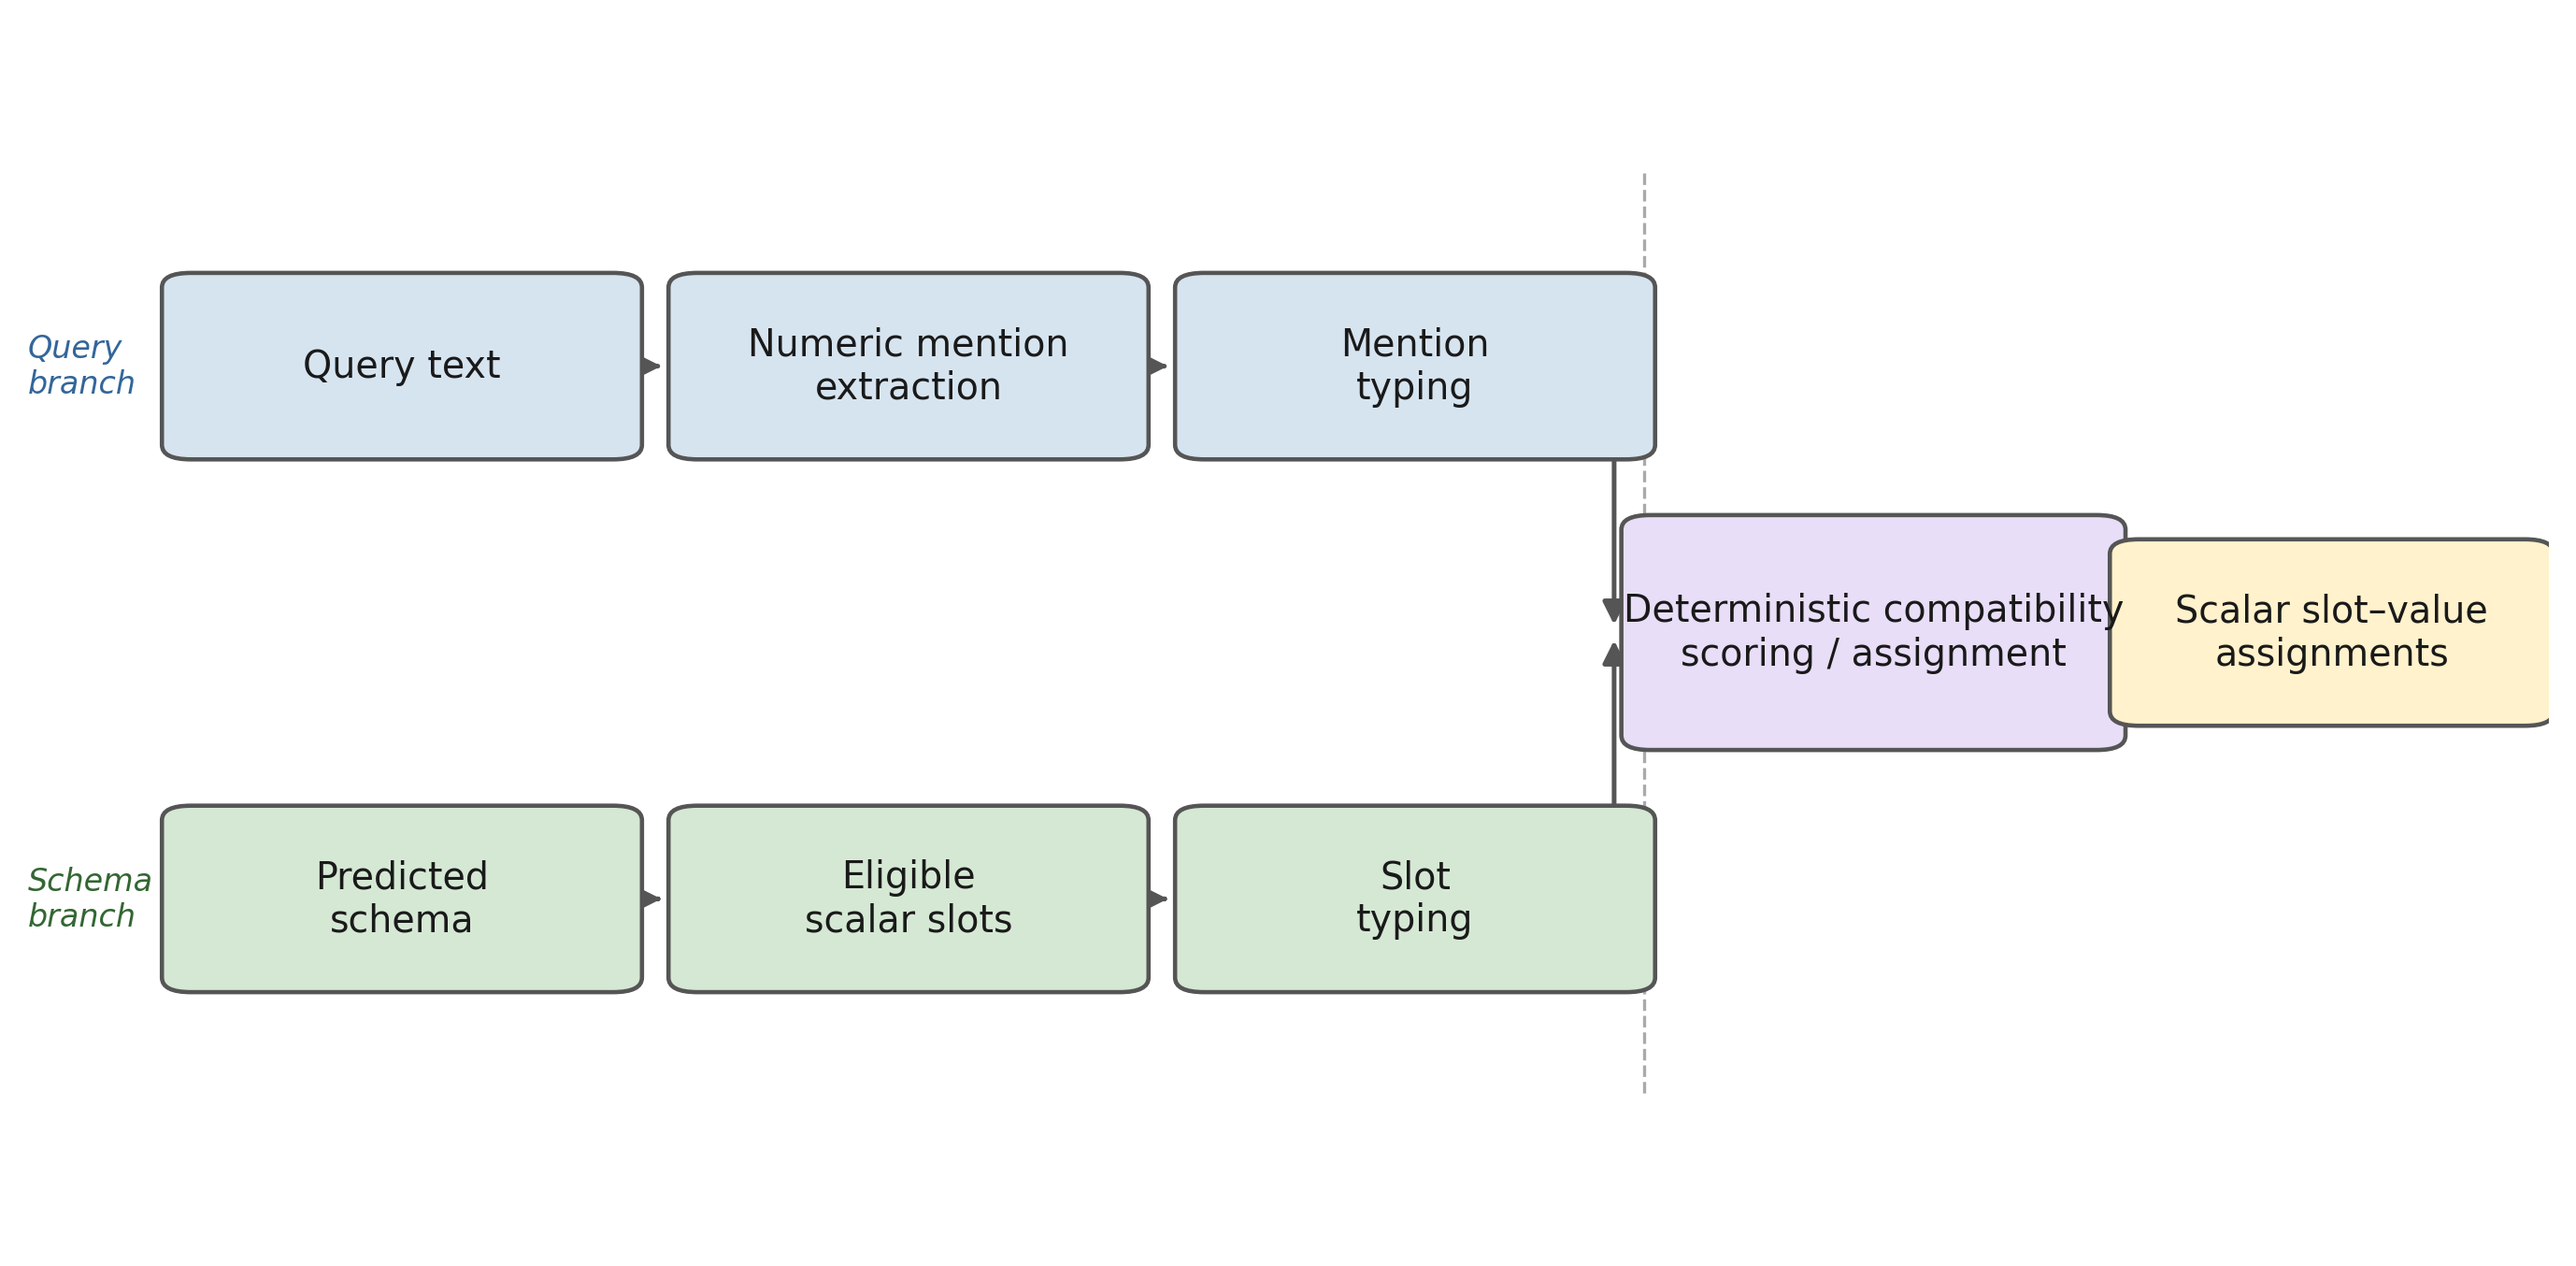
\includegraphics[width=0.82\linewidth]{figures/nlp4lp_instantiation_pipeline_v2.png}
  \caption{Schema-conditioned deterministic parameter instantiation. Numeric mentions are extracted from the query, typed using surface cues, filtered through the scalar slot inventory of the predicted schema, and assigned by a no-reuse compatibility rule. Alternative deterministic compatibility rules can be layered on this backbone.}
  \label{fig:instantiation-pipeline}
\end{figure}

\subsection{Evaluation-Oriented Design Choices}
\label{subsec:method_design}

Eligible slots are taken from the \emph{predicted} schema, not the gold schema, so retrieval errors propagate into coverage and readiness without using gold information to choose which schema is instantiated. Scalar-only evaluation provides a common substrate across templates (Section~\ref{subsec:method_problem}). Oracle and random references retain the interpretive roles in Section~\ref{subsec:method_retrieval}; the oracle is a control rather than a formal upper bound, because InstantiationReady need not be monotonic in schema correctness (Section~\ref{subsec:exp_engineering} reports a non-monotonic case on the 20-instance solver subset). Core metrics are solver-free and grounding is deterministic; executability is examined separately on restricted subsets. InstantiationReady is a diagnostic readiness criterion, not a guarantee of model correctness or solver compatibility.

\section{Experiments}
\label{sec:experiments}

\subsection{Experimental Setup}
\label{subsec:exp_setup}

We evaluate on \textsc{NLP4LP} \cite{nlp4lp_dataset,ahmaditeshnizi2024optimus_icml}, a curated gated public benchmark of LP/MILP descriptions pairing each instance with a gold parameter record and reference solver code. Unless noted, results use the 331-query test split; each query has one gold schema and is ranked against the 335-document catalog (random top-1 chance $1/335 \approx 0.0030$). Three query variants probe robustness: \emph{orig} (full text), \emph{noisy} (controlled lexical corruption and numeric masking), and \emph{short} (first sentence only).

Retrieval uses BM25, TF--IDF, LSA, and off-the-shelf BGE-M3 (no benchmark fine-tuning); only top-1 schemas enter grounding, with an oracle control for perfect selection. Downstream grounding follows Section~\ref{subsec:method_instantiation}, restricted to scalar slots induced by the predicted schema. Reported configurations are: (i)~TF--IDF typed-greedy with baseline extraction; (ii)~TF--IDF typed-greedy with ratio-aware extraction; (iii)~BGE-M3 with the same ratio-aware grounding; (iv)~oracle typed-greedy. Comparing (ii) and (iii) holds grounding fixed and varies only retrieval.

\textit{Schema R@1} is the fraction of queries with correct top-1 schema. For downstream metrics, let $G_i$ be eligible scalar gold slots after intersecting gold scalars with predicted-schema slots, and $A_i \subseteq G_i$ the assigned subset. Then
\begin{equation}
\textit{Coverage}
=
\frac{\sum_i |A_i|}{\sum_i |G_i|},
\label{eq:coverage}
\end{equation}
\begin{equation}
\textit{TypeMatch}
=
\frac{\sum_i |\{s \in A_i : \tau_{\mathrm{pred}}(i,s) = \tau_{\mathrm{slot}}(s)\}|}{\sum_i |A_i|},
\label{eq:typematch}
\end{equation}
where $\tau_{\mathrm{pred}}$ and $\tau_{\mathrm{slot}}$ are the mention and slot coarse types. \textit{Exact20 (on hits)} is computed only on schema-hit queries with a comparable predicted/gold numeric pair, using
\begin{equation}
\mathrm{error}(i,s) = \frac{|\hat{y}_{i,s} - y_{i,s}|}{\max(1.0, |y_{i,s}|)},
\label{eq:bounded_error}
\end{equation}
and counting a slot correct if $\mathrm{error}(i,s) \leq 0.20$. The denominator is method-dependent (main table: 291/291/303/320 comparable pairs for TF--IDF baseline, TF--IDF ratio-aware, BGE-M3, and Oracle), so Oracle need not dominate TF--IDF on this conditional metric. Exact20 is a conditional value-grounding measure; later sections rely on this definition.

\textit{InstantiationReady} uses per-query rates over $E(q_i,\hat{s}_i)$ (Eq.~\eqref{eq:eligible_slots}): $\mathit{Coverage}_i = |A_i|/|E|$ (0 if $E=\emptyset$) and $\mathit{TypeMatch}_i = |\{s\in A_i:\tau_{\mathrm{pred}}=\tau_{\mathrm{slot}}\}|/|A_i|$ (0 if $A_i=\emptyset$), with
\begin{equation}
\mathit{InstantiationReady}_i = \mathbb{1}\!\left[\mathit{Coverage}_i \geq 0.8 \ \wedge\ \mathit{TypeMatch}_i \geq 0.8\right].
\label{eq:instantiation_ready}
\end{equation}
The reported score is the mean over the 331-query denominator. The 0.8/0.8 threshold is a fixed diagnostic criterion; exact schema match is not a hard gate here (see StrictInstantiationReady in Section~\ref{subsec:exp_significance}).

Unless noted, retrieval and readiness metrics use the full denominator; Exact20 is the sole conditional exception. Paired significance uses a percentile bootstrap with $B=10{,}000$ resamples and seed $42$, plus exact McNemar tests where noted (Section~\ref{subsec:exp_significance}). We also report overlap sanitization diagnostics, the numeric-extraction ablation (Section~\ref{subsec:exp_error}), and three restricted structural/solver studies (Section~\ref{subsec:exp_engineering}). Table~\ref{tab:exp_blocks} summarizes blocks. Classical retrieval and grounding are CPU-compatible; BGE-M3 used GPU float32 L2-normalized 1024-d embeddings and cosine similarity without fine-tuning (Hugging Face \texttt{datasets} \cite{lhoest2021datasets}, \textsc{scikit-learn} \cite{pedregosa2011sklearn}). Implementation-level commands remain in the repository reproducibility map.

\begin{table}[t]
\centering
\caption{Summary of the experimental blocks used in the paper.}
\label{tab:exp_blocks}
\small
\begin{tabularx}{\linewidth}{X X X}
\toprule
Block & Primary purpose & Main outputs \\
\midrule
Main benchmark & Retrieval and scalar grounding on \textsc{NLP4LP} & Schema R@1, Coverage, TypeMatch, Exact20 (on hits), InstantiationReady \\
Robustness analyses & Sensitivity to degraded input and lexical overlap & Orig / noisy / short retrieval comparisons, overlap-based stress tests \\
Numeric-extraction ablation & Isolate effect of corrected ratio-word extraction & TypeMatch and InstantiationReady changes (baseline vs.\ ratio-aware extraction) \\
Significance testing & Assess whether reported gaps are statistically robust & Paired bootstrap $p$-values and confidence intervals \\
Structural validation (60 inst.) & Assess downstream structural usefulness & Structural-validity and instantiation-completeness rates \\
Extended structural validation (269 inst.) & Assess structural behavior on a larger subset with available reference code & Schema hit, structural validity, and instantiation completeness \\
Restricted solver-backed execution (20 inst.) & Real, restricted solver execution via SciPy HiGHS shim & Executable, solver-success, feasible, and objective-produced rates \\
\bottomrule
\end{tabularx}
\end{table}

\subsection{Schema Retrieval Performance}
\label{subsec:exp_retrieval}

Table~\ref{tab:nlp4lp-retrieval-main} reports Schema R@1 across query variants for the 335-way catalog (random chance $\approx 0.0030$). Within this fixed catalog---not as an open-domain claim---retrieval is already strong: BGE-M3 reaches $0.9456$ on orig versus TF--IDF $0.9094$ (McNemar $p=0.0075$; 15 BGE-only vs.\ 3 TF--IDF-only discordant wins). Noisy results remain close to orig; short truncations drop all methods but keep them well above chance (BGE-M3 $0.8157$). Average ranks: BGE-M3 $0.9013$, TF--IDF $0.8641$, BM25 $0.8469$, LSA $0.8328$. We retain TF--IDF as the primary lexical downstream backbone and also evaluate BGE-M3 downstream to test whether residual grounding difficulty persists under stronger retrieval. Absolute levels therefore set the paper's interpretive baseline: in this catalog, scalar grounding is the larger residual challenge.

\begin{table}[t]
  \centering
  \caption{Schema retrieval accuracy across query variants, reported as \textit{Schema R@1}. Each value is computed over all 331 test queries in the corresponding variant. The random baseline is the theoretical top-1 chance rate under uniform schema selection over the 335 candidate schemas, i.e., $1/335 \approx 0.0030$. Best result in each column is shown in bold.}
  \label{tab:nlp4lp-retrieval-main}
  \small
  \begin{tabular}{lcccc}
    \toprule
    Baseline & Orig & Noisy & Short & Avg. \\
    \midrule
    Random  & 0.0030 & 0.0030 & 0.0030 & 0.0030 \\
    LSA     & 0.8459 & 0.8882 & 0.7644 & 0.8328 \\
    BM25    & 0.8822 & 0.8912 & 0.7674 & 0.8469 \\
    TF--IDF & 0.9094 & 0.9033 & 0.7795 & 0.8641 \\
    BGE-M3 (dense) & \textbf{0.9456} & \textbf{0.9426} & \textbf{0.8157} & \textbf{0.9013} \\
    \bottomrule
  \end{tabular}
\end{table}

\subsection{Downstream Utility for Problem Instantiation}
\label{subsec:exp_downstream}

On the original queries, scalar-grounding outcomes follow the pattern in Table~\ref{tab:nlp4lp-downstream-main}. TF--IDF with ratio-aware extraction reaches Coverage $0.8886$, TypeMatch $0.8665$, and InstantiationReady $0.8006$; BGE-M3 with the same grounding improves InstantiationReady to $0.8248$ (Strict $0.8006$). TF--IDF ratio-aware remains strongest on Exact20 (on hits) at $0.2614$. Adding the schema gate (Eq.~\eqref{eq:strict_instantiation_ready}) lowers TF--IDF ratio-aware readiness from $0.8006$ to Strict $0.7704$, so a modest number of wrong-schema queries still meet ordinary thresholds. Replacing TF--IDF with BGE-M3 or with Oracle-TG (InstantiationReady $0.8489$) confirms that retrieval helps but does not close the gap: residual difficulty is value-to-slot grounding. Exact20 ordering (BGE-M3 $0.2436$, Oracle $0.2505$) reflects method-dependent denominators (Section~\ref{subsec:exp_setup}), not a claim that weaker retrieval improves value accuracy. These results characterize the restricted intermediate task, not full semantic understanding or open-domain model recovery.

\begin{table}[t]
  \centering
  \caption{Main downstream results on the original queries, computed from the final evaluation records. \textit{Coverage}, \textit{TypeMatch}, \textit{InstantiationReady}, and \textit{StrictInstantiationReady} use the full 331-query denominator. \textit{Exact20} (on hits) is conditional on schema-hit cases with comparable predicted and gold numeric values. Best non-oracle result in each column is shown in bold.}
  \label{tab:nlp4lp-downstream-main}
  \small
  \setlength{\tabcolsep}{3.2pt}
  \renewcommand{\arraystretch}{1.12}
  \begin{tabular}{@{}lccccc@{}}
    \toprule
    Method & Coverage & TypeMatch & Exact20 & InstReady & Strict \\
    \midrule
    TFIDF-TG (baseline extr.) & 0.8794 & 0.8515 & 0.2449 & 0.7764 & 0.7462 \\
    TFIDF-TG (ratio-aware extr.) & 0.8886 & 0.8665 & \textbf{0.2614} & 0.8006 & 0.7704 \\
    BGE-M3 + ratio-aware & \textbf{0.9154} & \textbf{0.8946} & 0.2436 & \textbf{0.8248} & \textbf{0.8006} \\
    Oracle-TG & 0.9416 & 0.9230 & 0.2505 & 0.8489 & 0.8489 \\
    \bottomrule
  \end{tabular}

  \vspace{2mm}
  \raggedright
  \footnotesize
  Abbreviations: TFIDF-TG = TF--IDF typed-greedy grounding; Oracle-TG = oracle schema selection with typed-greedy grounding; BGE-M3 = pretrained dense text encoder. All values are supported by the accompanying repository artifacts. \textit{Exact20 (on hits)} uses a single, uniformly applied denominator convention across all four rows: the mean of the per-query bounded-error indicator (Eq.~\eqref{eq:bounded_error}) over exactly the schema-hit queries that have a comparable predicted/gold numeric value, excluding (not zero-filling) schema-hit queries with no comparable value. The four rows accordingly condition on 291, 291, 303, and 320 comparable queries, respectively.
\end{table}

\subsection{Matched Same-Task Grounding Baselines}
\label{subsec:exp_grounding_baselines}

Under fixed TF--IDF retrieval, Table~\ref{tab:nlp4lp-grounding-baselines} compares predeclared, mechanism-diverse grounding alternatives on the same 331 queries and catalog, using shared InstantiationReady and Exact20 definitions and no tuning on test labels. Typed greedy and constrained assignment share the ratio-aware extractor; other rows use intrinsic enriched extractors required by their scoring definitions. Typed greedy remains best on InstantiationReady ($0.8006$) and StrictInstantiationReady ($0.7704$); all alternatives are significantly worse on InstantiationReady (paired bootstrap $B=10{,}000$, seed $42$; $p\leq 0.0006$), with McNemar likewise favoring typed greedy on Strict. Higher Exact20 for some alternatives (e.g., search-structured $0.6397$) comes with lower Coverage---an abstention tradeoff, not a reason to replace the production method.

\begin{table}[t]
  \centering
  \caption{Matched same-task grounding baselines on the $331$ original queries with TF--IDF retrieval held fixed. Only the grounding/assignment mechanism changes. Best InstantiationReady / StrictInstantiationReady values are shown in bold.}
  \label{tab:nlp4lp-grounding-baselines}
  \small
  \setlength{\tabcolsep}{2.8pt}
  \renewcommand{\arraystretch}{1.12}
  \begin{tabular}{@{}lccccc@{}}
    \toprule
    Grounding method & Coverage & TypeMatch & Exact20 & InstReady & Strict \\
    \midrule
    Typed greedy (production) & 0.8886 & 0.8665 & 0.2614 & \textbf{0.8006} & \textbf{0.7704} \\
    Constrained assignment & 0.8531 & 0.8745 & 0.5772 & 0.7613 & 0.7311 \\
    Max-weight matching & 0.8436 & 0.8740 & 0.5225 & 0.7432 & 0.7130 \\
    Optimization-role repair & 0.8436 & 0.8724 & 0.5210 & 0.7372 & 0.7069 \\
    Search-structured grounding & 0.8195 & 0.8795 & 0.6397 & 0.7039 & 0.6737 \\
    Semantic-IR repair & 0.8131 & 0.8483 & 0.4949 & 0.7160 & 0.6949 \\
    \bottomrule
  \end{tabular}

  \vspace{2mm}
  \raggedright
  \footnotesize
  Typed greedy and constrained assignment share the final ratio-aware extractor; the other rows use their intrinsic enriched extractors as part of their grounding definitions. \textit{Exact20 (on hits)} denominators are 291 comparable schema-hit queries for all rows except semantic-IR repair (285), under the same exclude-noncomparable convention as Table~\ref{tab:nlp4lp-downstream-main}.
\end{table}

\subsection{Error Analysis and Ablation Studies}
\label{subsec:exp_error}

A mutually exclusive residual-error decomposition on all 331 orig queries (Table~\ref{tab:nlp4lp-error-taxonomy}; fixed category order, one label each) for TF--IDF ratio-aware typed greedy yields: wrong schema $30$ ($9.1\%$); incomplete coverage $31$ ($9.4\%$); type mismatch $49$ ($14.8\%$); value inaccurate $214$ ($64.7\%$); fully correct $7$ ($2.1\%$). Counts are deterministic from frozen per-query records. The dominant residual is fine-grained value-to-slot correctness among type-compatible mentions---the ambiguity Exact20 (Section~\ref{subsec:exp_setup}) targets---not coarse typing or retrieval.

The ratio-word extraction ablation in Table~\ref{tab:nlp4lp-prefix-postfix} raises Coverage from $0.8794$ to $0.8886$, TypeMatch from $0.8515$ to $0.8665$, InstantiationReady from $0.7764$ to $0.8006$, and Strict from $0.7462$ to $0.7704$ (8 strict gains, 0 losses; McNemar $p=0.008$). Retrieval is unchanged. Gains are real but modest; the remaining oracle gap reflects semantic ambiguities (totals vs.\ unit coefficients, bounds, percent vs.\ absolute values) rather than the extraction patch.

\begin{table}[t]
  \centering
  \caption{Mutually exclusive residual-error decomposition for TF--IDF ratio-aware typed greedy on 331 orig queries (fixed category order; counts sum to 331).}
  \label{tab:nlp4lp-error-taxonomy}
  \small
  \setlength{\tabcolsep}{4pt}
  \begin{tabular}{p{7.4cm}cc}
    \toprule
    Category & Count & Fraction \\
    \midrule
    Wrong schema (schema retrieval fails) & 30 & 0.091 \\
    Incomplete coverage (correct schema, $\geq 1$ slot unfilled) & 31 & 0.094 \\
    Type mismatch (correct schema, full coverage, $\geq 1$ wrong type) & 49 & 0.148 \\
    Value inaccurate (correct schema, full coverage, correct types, $\geq 1$ value outside tolerance) & 214 & 0.647 \\
    Fully correct (all four criteria satisfied) & 7 & 0.021 \\
    \midrule
    Total & 331 & 1.000 \\
    \bottomrule
  \end{tabular}
\end{table}

\begin{table}[t]
  \centering
  \caption{Numeric-extraction ablation on the original queries, comparing the baseline and ratio-aware extraction configurations of the TF--IDF typed-greedy method. The ratio-aware configuration corrects multiplicative ratio-word numeric expressions. The strict-ready count (of 331) rises from 247 to 255; see Section~\ref{subsec:exp_significance} for the significance test.}
  \label{tab:nlp4lp-prefix-postfix}
  \small
  \setlength{\tabcolsep}{4pt}
  \begin{tabular}{lccc}
    \toprule
    Metric & Baseline & Ratio-aware & $\Delta$ \\
    \midrule
    Coverage & 0.8794 & 0.8886 & +0.0092 \\
    TypeMatch & 0.8515 & 0.8665 & +0.0150 \\
    Exact20 (on hits) & 0.2449 & 0.2614 & +0.0165 \\
    InstantiationReady & 0.7764 & 0.8006 & +0.0242 \\
    StrictInstantiationReady & 0.7462 & 0.7704 & +0.0242 \\
    \bottomrule
  \end{tabular}
\end{table}

\subsection{Statistical Significance and Lexical-Overlap Robustness}
\label{subsec:exp_significance}

Paired bootstrap tests on orig queries ($B=10{,}000$, seed $42$; Table~\ref{tab:nlp4lp-significance}) show that the TF--IDF ratio-aware versus Oracle InstantiationReady and Strict gaps are significant; the ratio-aware strict gain ($\Delta=+0.0242$; McNemar $p=0.008$) and the BGE-M3 versus TF--IDF InstantiationReady/Strict gains are likewise significant.

Lexical-overlap sanitization (Table~\ref{tab:nlp4lp-overlap}) shows that stripping numbers and/or stopwords does not destroy lexical retrieval; performance is preserved or improved, consistent with reliance on domain terms rather than numeric literals. The diagnostic uses a closely matched index (331 documents excluding four filler templates; no \texttt{doc\_id} tokens), so TF--IDF/BM25 baseline cells differ slightly from Table~\ref{tab:nlp4lp-retrieval-main} while LSA matches exactly ($0.8459$). A Jaccard-overlap stratification places 327/331 queries in a high-overlap bucket (TF--IDF R@1 $0.9174$); the medium-overlap bucket has only 4 queries and is reported only as a qualitative caveat.

To check whether wrong schemas can inflate ordinary InstantiationReady via smaller eligible-slot sets, a repository diagnostic of selective schema reranking raised ordinary readiness from $257/331$ to $265/331$, but $6$ of $8$ newly ready queries used an incorrect schema. We therefore define
\begin{equation}
\mathit{StrictInstantiationReady}_i = \mathbb{1}\!\left[\mathit{SchemaHit}_i \wedge \mathit{Coverage}_i \geq 0.8 \wedge \mathit{TypeMatch}_i \geq 0.8\right],
\label{eq:strict_instantiation_ready}
\end{equation}
as a robustness check (Table~\ref{tab:strict-instready}). The gate removes 10 TF--IDF queries in both extraction configurations and widens the TF--IDF--Oracle InstantiationReady gap from $0.0483$ to $0.0785$ ($p<0.001$), without changing the qualitative conclusion.

\begin{table}[t]
\centering
\caption{Paired bootstrap significance tests ($B=10{,}000$ resamples, original queries) computed from the final per-query evaluation records. Diff is method A minus method B on the stated metric.}
\label{tab:nlp4lp-significance}
\small
\setlength{\tabcolsep}{2.5pt}
\begin{tabular}{@{}p{0.50\linewidth}ccc@{}}
  \toprule
  Comparison (metric) & Diff & 95\% CI & $p$ \\
  \midrule
  TFIDF-TG (ratio) vs.\ Oracle-TG (InstReady) & $-0.0483$ & $[-0.0755,\,-0.0242]$ & $<0.001$ \\
  TFIDF-TG (ratio) vs.\ Oracle-TG (Strict) & $-0.0785$ & $[-0.1088,\,-0.0514]$ & $<0.001$ \\
  TFIDF-TG baseline vs.\ ratio (Strict) & $+0.0242$ & $[0.0091,\,0.0423]$ & $0.0006$ \\
  BGE-M3 vs.\ TFIDF-TG (ratio) (InstReady) & $+0.0242$ & $[0.0060,\,0.0423]$ & $0.0053$ \\
  BGE-M3 vs.\ TFIDF-TG (ratio) (Strict) & $+0.0302$ & $[0.0060,\,0.0544]$ & $0.0142$ \\
  \bottomrule
\end{tabular}

\vspace{2mm}
\raggedright
\footnotesize
The baseline versus ratio-aware extraction comparison (8 strict gains, 0 losses) is also significant under an exact McNemar test ($p=0.008$). CI = confidence interval. ``ratio'' abbreviates the ratio-aware extraction configuration. All five rows are reproducible from a single committed, deterministic script (paired percentile bootstrap, $B=10{,}000$, seed $42$, two-sided $p=2\min(P(\Delta\leq 0),P(\Delta>0))$ over the bootstrap resamples) applied to the frozen per-query records; see Code availability.
\end{table}

\begin{table}[t]
\centering
\caption{Retrieval accuracy (\textit{Schema R@1}, original queries) after removing numeric tokens and/or stopwords, using the diagnostic sanitization configuration with 256-dimensional LSA. The TF--IDF and BM25 baseline rows differ slightly from the canonical Table~\ref{tab:nlp4lp-retrieval-main} evaluation because of the catalog and indexed-document configuration differences described in the text; the LSA baseline reproduces the Table~\ref{tab:nlp4lp-retrieval-main} value exactly.}
\label{tab:nlp4lp-overlap}
\small
\begin{tabular}{lccc}
  \toprule
  Sanitization & TF--IDF & BM25 & LSA \\
  \midrule
  None (baseline)               & 0.9063 & 0.8852 & 0.8459 \\
  Numbers removed               & 0.9063 & 0.8973 & 0.8459 \\
  Stopwords removed             & 0.9124 & 0.9063 & 0.9184 \\
  Numbers \& stopwords removed  & 0.9124 & 0.9063 & 0.9184 \\
  \bottomrule
\end{tabular}
\end{table}

\begin{table}[t]
\centering
\caption{Sensitivity check: canonical \textit{InstantiationReady} versus the stricter \textit{StrictInstantiationReady} (Eq.~\eqref{eq:strict_instantiation_ready}), original queries, computed from the final per-query evaluation records. $\Delta$ is standard minus strict; $n_{\text{differ}}$ counts queries whose readiness label changes.}
\label{tab:strict-instready}
\small
\begin{tabular}{lcccc}
  \toprule
  Method & InstReady & StrictInstReady & $\Delta$ & $n_{\text{differ}}$ \\
  \midrule
  TFIDF-TG (baseline) & 0.7764 & 0.7462 & 0.0302 & 10 \\
  TFIDF-TG (ratio-aware) & 0.8006 & 0.7704 & 0.0302 & 10 \\
  Oracle-TG & 0.8489 & 0.8489 & 0.0000 & 0 \\
  \bottomrule
\end{tabular}
\end{table}

\subsection{Computational Complexity and Runtime}
\label{subsec:exp_runtime}

The deterministic backbone is inexpensive on this catalog. TF--IDF fits a sparse vectorizer once over the $M=335$ schema documents and, for each query, transforms the query and scores it against the full catalog matrix by sparse cosine similarity (\textsc{scikit-learn}); with fixed small $M$, this is dominated by sparse vector arithmetic rather than any learned inference. Rule-based extraction is linear in query length. Typed-greedy assignment costs $O(|\mathcal{P}|\cdot|\mathcal{T}|)$ in the (typically small) numbers of eligible slots and mentions. On the frozen TF--IDF + ratio-aware typed-greedy run (331 queries, one CPU core, \texttt{PYTHONHASHSEED=0}), wall time is $1.09$\,s ($3.29$\,ms/query) with peak RSS $\approx 198$\,MB. This excludes BGE-M3 embedding load/compute and remote LLM baselines; it substantiates that the deterministic backbone is lightweight and CPU-compatible, not a cross-method efficiency benchmark.

\subsection{Structural and Solver-Backed Validation}
\label{subsec:exp_engineering}

Core metrics are solver-free. We complement them with three restricted studies on subsets that have available reference solver code (\texttt{optimus\_code}): static structural analyses on 60 and 269 instances (no Gurobi required) and solver-backed execution on 20 HiGHS-compatible instances via a SciPy HiGHS compatibility shim. All three are restricted by construction and do not claim benchmark-wide executability.

We define the validation metrics as per-instance Boolean conditions, each reported as a rate over the relevant subset. \emph{Structural validity} holds when the instantiated schema forms a well-formed linear or mixed-integer program with a defined objective and at least one decision variable, checked statically without invoking a solver. \emph{Instantiation completeness} holds when every scalar slot the gold schema marks as required receives a type-consistent assignment. \emph{Executable} holds when the generated solver program runs to completion without raising an exception. \emph{Solver success} holds when the solver returns a well-defined termination status rather than erroring. \emph{Feasible} holds when the solver reports a feasible solution, and \emph{objective produced} holds when it returns a finite objective value. Structural validity and instantiation completeness are static checks; the remaining four require executing the solver.

\paragraph{Structural subset (60 instances)}
Table~\ref{tab:eng-structural} reports schema-hit, structural-validity, and instantiation-completeness rates. TF--IDF reaches structural-valid and instantiation-complete rates of $0.75$; Oracle reaches $0.7667$ and $0.7833$. As in the main benchmark, the oracle gain over TF--IDF is small: schema selection helps only modestly, while substantial downstream limitations remain.

\begin{table}[t]
\centering
\caption{Structural subset (60 instances): schema-hit, structural-validity, and instantiation-completeness rates.}
\label{tab:eng-structural}
\small
\begin{tabular}{lccc}
  \toprule
  Baseline & Schema Hit & Structural Valid & Inst.\ Complete \\
  \midrule
  TF--IDF & 0.9333 & 0.7500 & 0.7500 \\
  BM25    & 0.9000 & 0.7333 & 0.7333 \\
  Oracle  & 1.0000 & 0.7667 & 0.7833 \\
  \bottomrule
\end{tabular}
\end{table}

\paragraph{Extended structural subset (269 instances)}
On a larger subset with available reference solver code, TF--IDF, BM25, and Oracle achieve schema-hit rates of $0.9368$, $0.9257$, and $1.0000$; structural-validity rates of $0.8141$, $0.8104$, and $0.8253$; and instantiation-completeness rates of $0.6654$, $0.6580$, and $0.6840$. Solver execution was not evaluated here because the reference path required Gurobi support unavailable in the evaluation environment; executable conclusions are reserved for the HiGHS-compatible subset below.

\paragraph{Restricted solver-backed subset (20 instances)}
To obtain direct solver-backed evidence, we select the first 20 test-split instances whose gold \texttt{optimus\_code} lacks unsupported commercial constructs (e.g., piecewise-linear objectives or specialized API constraints) under a fixed, outcome-independent compatibility filter. The same 20 IDs are used for TF--IDF and Oracle and were fixed before evaluating either condition. Table~\ref{tab:eng-solver} reports executable, solver-success, feasible, and objective-produced rates: TF--IDF reaches $0.95$ executable and $0.80$ on the three solver-outcome rates; Oracle reaches $0.95$, $0.75$, $0.75$, and $0.75$. Non-executions are shim \texttt{IndexError}s (2 of 40 baseline--instance evaluations). The $0.80$ versus $0.75$ gap is statistically inconclusive on this small, compatibility-filtered subset and should be read only as evidence that solver execution is possible on compatible cases, not as benchmark-wide readiness.

\begin{table}[t]
\centering
\caption{Restricted solver-backed subset (20 instances, SciPy HiGHS MILP compatibility shim; Gurobi not required).}
\label{tab:eng-solver}
\small
\begin{tabular}{lcccc}
  \toprule
  Baseline & Executable & Solver Success & Feasible & Objective Produced \\
  \midrule
  TF--IDF & 0.95 & 0.80 & 0.80 & 0.80 \\
  Oracle  & 0.95 & 0.75 & 0.75 & 0.75 \\
  \bottomrule
\end{tabular}
\end{table}

Across subsets, Oracle does not consistently dominate TF--IDF, matching the main-benchmark pattern that schema selection yields only modest gains while downstream limits remain. Extended-subset structural gaps (missing slots, type mismatch, and incomplete instantiation: 69, 82, and 267 counted instances across baselines) align with Section~\ref{subsec:exp_error}.

\subsection{External Baseline Comparison on a Shared Subset}
\label{subsec:exp_external}

The proposed method performs fixed-catalog scalar grounding and does not emit complete formulations or solver code. Its native InstantiationReady / Exact20 metrics are therefore not numerically comparable to end-to-end LLM modeling systems, and Tables~\ref{tab:ext-context}--\ref{tab:ext-outcomes} should be read as contextual common-18 evidence under a shared harness rather than as a leaderboard (full per-instance protocol in the repository).

Several fairness qualifications follow. PaMOP is an independent Azure OpenAI reconstruction (\texttt{gpt-5.4-2026-03-05}, evaluated 2026-08-15, temperature $0.2$), with objective agreement defined as a $5\%$ relative tolerance on evaluable successful runs. ORLM execution is marked N/A because its \texttt{coptpy} solver dependency was unavailable. DeepOR has no located official code or checkpoint, and OR-R1 publishes code without a released checkpoint, so neither yields an evaluable artifact. The generic LLM is a zero-shot harness baseline (temperature $0.0$), not an optimization-trained method, and must not be ranked against OptMATH's official checkpoint (temperature $0.8$). Finally, $n=18$ is a feasibility probe: the proposed method is excluded from every shared end-to-end cell in Table~\ref{tab:ext-outcomes} because the tasks differ.

\begin{table}[t]
  \centering
  \caption{External-baseline provenance on the common-18 subset. Provenance levels: NATIVE, INDEPENDENT, ADAPTED-OFFICIAL, GENERIC-ZERO-SHOT. Ours is listed for context only; native metrics are not comparable to Table~\ref{tab:ext-outcomes}.}
  \label{tab:ext-context}
  \small
  \setlength{\tabcolsep}{3pt}
  \renewcommand{\arraystretch}{1.15}
  \begin{tabular}{@{}>{\raggedright\arraybackslash}p{1.9cm}>{\raggedright\arraybackslash}p{2.6cm}>{\raggedright\arraybackslash}p{2.5cm}>{\raggedright\arraybackslash}p{3.55cm}c@{}}
    \toprule
    System & Provenance & Output representation & Solver environment / status & Cases \\
    \midrule
    Ours (this paper) & NATIVE & Scalar slot assignments on retrieved schema & No solver call in core benchmark & 18 \\
    PaMOP \cite{pan2025pamop} & INDEPENDENT & AMPL formulation + solver code & Local AMPL + HiGHS; 13/18 executed & 18 \\
    ORLM \cite{huang2025orlm} & ADAPTED- OFFICIAL & LP formulation + solver code & Solver dependency (\texttt{coptpy}) unavailable; execution blocked & 18 \\
    OptMATH \cite{lu2025optmath} & ADAPTED- OFFICIAL & LP formulation + solver code & Gurobi (\texttt{gurobipy}); 15/18 executed & 18 \\
    Generic LLM (GPT-5.4- 2026-03-05) & GENERIC- ZERO-SHOT & Gurobi solver code, zero-shot & Gurobi (\texttt{gurobipy}); 16/18 executed & 18 \\
    DeepOR \cite{xiao2026deepor} & --- & Formulation (paper-described) & No official code or released checkpoint located; no evaluable artifact exists & 0 \\
    OR-R1 \cite{ding2026orr1} & --- & Formulation + solver code & Official code public; no checkpoint released; execution not possible & 0 \\
    \bottomrule
  \end{tabular}
\end{table}

\begin{table}[t]
  \centering
  \caption{Shared outcomes on the 18-instance common subset. N/A = not evaluated (never a silent zero). \textit{Parse}: fraction whose produced artifact parsed; \textit{Executable}: fraction whose solver code ran to completion; \textit{Feasible}: fraction of successful runs reporting a feasible solution; \textit{Objective agreement}: fraction of execution-successful cases with a comparable reference objective agreeing within $5\%$ relative tolerance. Denominators vary by stage reached.}
  \label{tab:ext-outcomes}
  \small
  \setlength{\tabcolsep}{4pt}
  \begin{tabular}{lcccc}
    \toprule
    System & Parse & Executable & Feasible & Objective agreement \\
    \midrule
    Ours (this paper) & N/A & N/A & N/A & N/A \\
    PaMOP \cite{pan2025pamop} & 0.72 & 0.72 & 1.00 & 0.73 (8/11) \\
    ORLM \cite{huang2025orlm} & 1.00 & N/A & N/A & N/A \\
    OptMATH \cite{lu2025optmath} & 1.00 & 0.83 & 1.00 & 0.40 (6/15) \\
    Generic LLM (GPT-5.4-2026-03-05) & 1.00 & 0.89 & 1.00 & 0.63 (10/16) \\
    \bottomrule
  \end{tabular}
\end{table}

\subsection{External Component-Level Robustness Validation}
\label{subsec:exp_external_validation}

As a component-level check, we evaluated numeric extraction on a fixed 1,000-instance \textsc{OptMATH}-Train sample \cite{lu2025optmath} (no fixed schema catalog, so extraction only). Raw AST code-value overlap recall is $0.7501$; automatic text-support recall $0.8118$ (complete-instance rate $0.5910$). A secondary rule-based classifier on 150 instances (seed 20260815) finds that $7.28\%$ of the AST denominator are implementation/loop/solver constants. Audit-calibrated text-supported recall is $0.8070$ (95\% CI $[0.7842,0.8283]$, $n=28{,}799$ auto-classified text-supported values). Two independently coded classifiers agree on $98.04\%$ of 4,801 literals in the 150-instance sample---automated cross-validation, not human gold labels. This is limited evidence that extraction transfers beyond \textsc{NLP4LP}; it does not establish full-framework generalization.

\section{Conclusions and Future Research}
\label{sec:conclusion}

We studied fixed-catalog schema retrieval paired with deterministic scalar grounding as an intermediate natural-language-to-optimization capability. On \textsc{NLP4LP}, lexical and dense retrieval are already strong; BGE-M3 improves InstantiationReady, yet the oracle gain remains modest, and residual-error analysis attributes most remaining failures to fine-grained value-to-slot correctness. Matched same-task grounding alternatives do not displace typed greedy on InstantiationReady/Strict. Restricted structural and solver-backed subsets suggest usefulness on compatible cases without establishing benchmark-wide solver readiness. Limitations are consolidated in Section~\ref{subsec:limitations}.

\subsection{Limitations and Threats to Validity}
\label{subsec:limitations}

\emph{Fixed-catalog retrieval and task scope.} Strong retrieval numbers characterize the 335-way NLP4LP catalog (Section~\ref{subsec:method_retrieval}) and must not be read as solving open-domain schema retrieval. Generalization to substantially larger or open-ended schema libraries remains untested.

\emph{Dataset dependence and lexical overlap.} All main quantitative results use a single benchmark. Overlap sanitization (Section~\ref{subsec:exp_significance}) argues against pure numeric-literal matching, but the medium-overlap bucket has only 4 queries, so cross-style, cross-domain, and cross-language generalization remains untested.

\emph{Gated data access.} NLP4LP requires approved Hugging Face access. Committed artifacts support inspection without live queries; a full end-to-end rerun needs the gated data, which is a real (if benchmark-typical) reproducibility constraint.

\emph{Scalar-only instantiation.} Coverage, TypeMatch, and InstantiationReady characterize scalar recovery only (Section~\ref{subsec:method_design}); they do not certify recovery of variables, constraints, or structured objects.

\emph{Heuristic type and role inference.} Coarse typing and optional role cues are rule-based without formal guarantees; Table~\ref{tab:nlp4lp-error-taxonomy} shows that value-to-slot ambiguity remains dominant even when coarse types are correct.

\emph{Restricted solver-backed validation.} Subsets of size 60 / 269 / 20 are availability- or compatibility-filtered rather than random samples; the HiGHS-only 20-case study cannot support benchmark-wide readiness claims (Section~\ref{subsec:exp_engineering}).

\emph{Limited end-to-end LLM comparison.} Related Work and the common-18 assessment contextualize OptiMUS, OptLLM, ORLM, OptMATH, OptimAI, AlphaOPT, ORThought, and others, but do not provide full-benchmark InstantiationReady head-to-heads; DeepOR and OR-R1 lack evaluable artifacts (Section~\ref{subsec:exp_external}).

\emph{No external full-framework validation or deployment.} OptMATH validates extraction only (Section~\ref{subsec:exp_external_validation}); no user study or production deployment was conducted.

\subsection{Future Research Directions}
\label{subsec:future_work}

Natural next steps include stronger semantic role-sensitive grounding, structured (non-scalar) parameters, hybrid retrieval-plus-learned/LLM grounding, and broader solver-backed coverage. Intermediate schema retrieval and schema-conditioned instantiation remain scientifically useful even while full automation stays difficult.


\backmatter

\section*{Declarations}

\noindent\textbf{Funding.} This research did not receive any specific grant from funding agencies in the public, commercial, or not-for-profit sectors. The external large-language-model baseline experiments used Microsoft Azure OpenAI services; associated usage was supported by the standard Azure for Students educational credit available to the author.

\noindent\textbf{Competing interests.} The author declares that there are no known competing financial interests or personal relationships that could have appeared to influence the work reported in this paper.

\noindent\textbf{Ethics approval and consent to participate.} Not applicable; this study did not involve human participants, human data, or animals.

\noindent\textbf{Author contributions.} Soroush Vahidi: Conceptualization, Methodology, Software, Validation, Formal analysis, Investigation, Data curation, Writing -- original draft, Writing -- review \& editing, Visualization. This single-author paper uses the standard CRediT taxonomy to describe the contributions of the sole author.

\noindent\textbf{Data availability.} The benchmark used in this paper, NLP4LP (\texttt{udell-lab/NLP4LP} on Hugging Face), is a gated third-party dataset. The author does not redistribute this dataset; eligible researchers must obtain it directly from its original Hugging Face source under its specific access conditions. The derived artifacts supporting the results reported in this paper, together with the corresponding tables, figures, and analysis outputs, are publicly available in the accompanying GitHub repository at \url{https://github.com/SoroushVahidi/combinatorial-opt-agent}.

\noindent\textbf{Code availability.} The retrieval, grounding, evaluation, and analysis code supporting this paper is available at \url{https://github.com/SoroushVahidi/combinatorial-opt-agent}. Reproducing a full NLP4LP rerun requires the gated dataset access described above.

\noindent\textbf{Declaration of generative AI and AI-assisted technologies in the writing process.} During the preparation of this work the author used ChatGPT and Gemini to improve readability and language. After using these tools, the author reviewed and edited the content as needed and takes full responsibility for the content of the published article.

\noindent\textbf{Declaration of AI assistance in software development.} During the research and software-development process, the author used Claude, Cursor, and GitHub Copilot for coding assistance. The author reviewed, verified, tested, and edited the resulting code and takes full responsibility for the implementation and reported results. Note that the scalar grounding procedure evaluated in this paper is deterministic at inference time and does not itself rely on generative LLM inference; schema retrieval is evaluated using both deterministic lexical methods and the pretrained BGE-M3 dense encoder (with the exception of the external baselines evaluated separately in Section~\ref{subsec:exp_external}).

\bibliography{references}

\end{document}
